% --
% intro

\section{Signal Processing and Feature Extraction}
\sectionheader{Signal Processing and Feature Extraction}
\begin{frame}
  \frametitle{Speech Signal}
  \begin{itemize}
    \item Signal with $N$ samples
    \begin{equation*}\label{eq:signal_raw_x}
      \footnotesize
      \bm{x} = [x_0, x_1, \dots, x_{N-1}]^T
    \end{equation*}
  \end{itemize}
  \begin{figure} 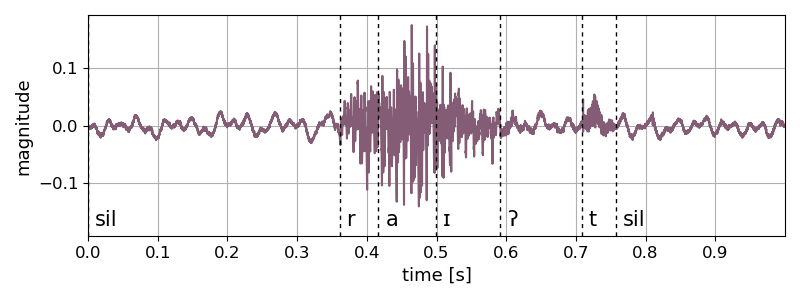
\includegraphics[width=0.8\textwidth]{../3_signal/figs/signal_raw_showcase_right0.png} \end{figure}
\end{frame}

\begin{frame}
  \frametitle{Spectral Features}
  \vspace{-0.5cm}
  \begin{itemize}
    \item Discrete Fourier Transform (DFT):
    \begin{equation*}\label{eq:signal_spec_dtft_matrix}
      \footnotesize
      \begin{aligned}
        \hat{\bm{x}} = \mathcal{F} \bm{x} \quad & \mathrm{with} 
        \quad \mathcal{F}[k, n] = e^{-j\frac{2 \pi n}{N} k},\\
        &k, n = (0, 1, \dots, K-1), (0, 1, \dots, N-1)
      \end{aligned}
    \end{equation*}

    \item Short-Time Fourier Transform (STFT):
    \begin{equation*}\label{eq:signal_spec_stft}
      \footnotesize
      \begin{aligned}
        \tilde{X}[k, m] &= \sum_{n=0}^{N-1} x[n + m h] \, w[n] \, e^{-j\frac{2 \pi n}{N}k},\\ 
        m &= 0, 1, \dots, M - 1,\\
        M &= \ceil*{\frac{\norm{\bm{x}}_0-N}{h}}
      \end{aligned}
    \end{equation*}
  \end{itemize}
\end{frame}

\begin{frame}
  \frametitle{Spectral Features}
  \vspace{-0.5cm}
  \begin{itemize}
    \item Spectrogram:
    \begin{equation*}
      \footnotesize
      P = \abs{\tilde{X}}^2
    \end{equation*}
  \end{itemize}
  \begin{figure} 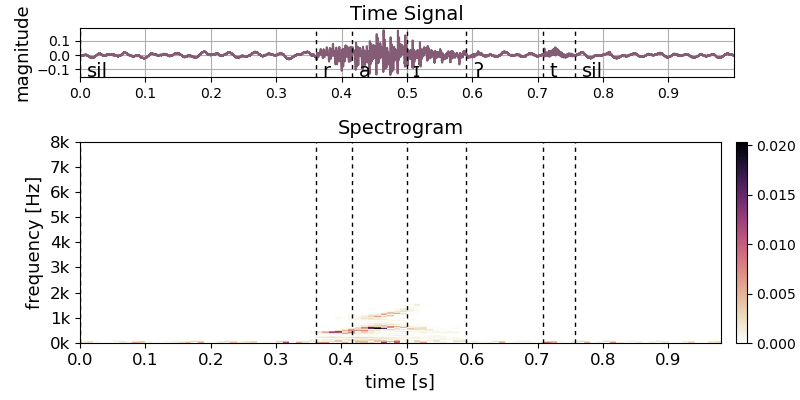
\includegraphics[width=0.8\textwidth]{../3_signal/figs/signal_spec-lin_showcase_right0.png} \end{figure}
\end{frame}

\begin{frame}
  \frametitle{Spectral Features}
  \vspace{-0.5cm}
  \begin{itemize}
    \item logarithmic Spectrogram:
    \begin{equation*}
      \footnotesize
      P_{DB} = 10 \cdot \log_{10}{P}
    \end{equation*}
  \end{itemize}
  \begin{figure} 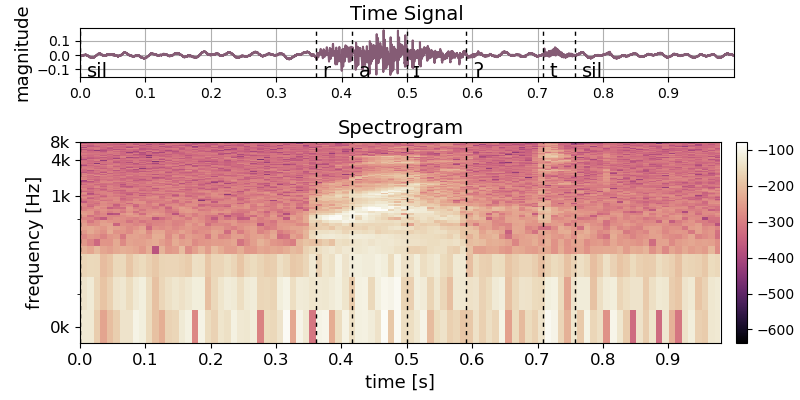
\includegraphics[width=0.8\textwidth]{../3_signal/figs/signal_spec-log_showcase_right0.png} \end{figure}
\end{frame}

\begin{frame}
  \frametitle{MFCC Features}
  \vspace{-0.5cm}
  \begin{itemize}
    \item MFCC:
    \begin{equation*}
      \footnotesize
      U = \mathcal{D} \log{ \left( W_m   P \right) }
    \end{equation*}
  \end{itemize}
  \begin{figure}
    \centering
    \subfigure[DCT ($\mathcal{D}$)]{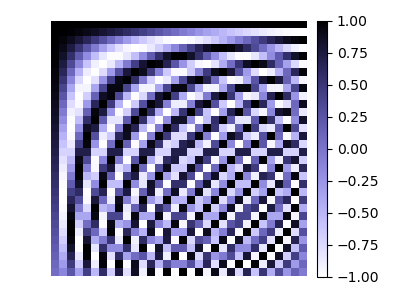
\includegraphics[width=0.45\textwidth]{../3_signal/figs/signal_mfcc_dct.png}}
    \subfigure[Mel Bands ($W_m$)]{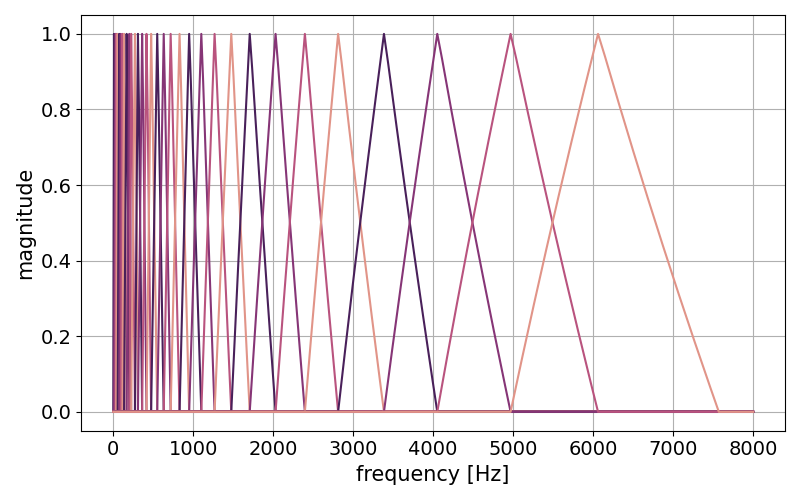
\includegraphics[width=0.5\textwidth]{../3_signal/figs/signal_mfcc_weights_f.png}}
  \end{figure}
\end{frame}

\begin{frame}
  \frametitle{MFCC Features}
  \vspace{-1cm}
  \begin{itemize}
    \item frame based normalization:
    \begin{equation*}
      \scriptsize
      \begin{aligned}
        &U[c, m] \gets \frac{U[c, m] + \vert \underset{m \in \mathcal{M}}{\min} \bm{u}_c \vert}{\norm{\bm{u}_c + \vert \underset{m \in \mathcal{M}}{\min} \bm{u}_c \vert}_\infty}\\
        & \forall \, c, m = (0, 1, \dots, C - 1), (0, 1, \dots, M - 1)
      \end{aligned}
    \end{equation*}
  \end{itemize}
  \vspace{-0.25cm}
  \begin{figure} 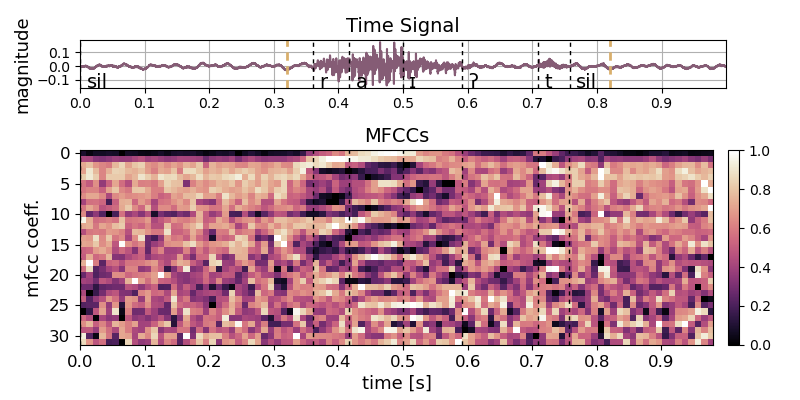
\includegraphics[width=0.8\textwidth]{../3_signal/figs/signal_mfcc_showcase_mfcc32_right0.png} \end{figure}
\end{frame}

\begin{frame}
  \frametitle{MFCC Feature Enhancements}
  \vspace{-1cm}
  \begin{itemize}
    \item Delta- and Double Delta Features:
    \begin{equation*}\label{eq:signal_mfcc_delta}
      \scriptsize
      \Delta u_c[m] = \frac{u_c[m - 1] + u_c[m + 1]}{2}
    \end{equation*}
    \item Energy Features:
    \begin{equation*}
      \scriptsize
      e[m] = \bm{u}[m]^T \bm{u}[m]
    \end{equation*}
  \end{itemize}
  \begin{figure} 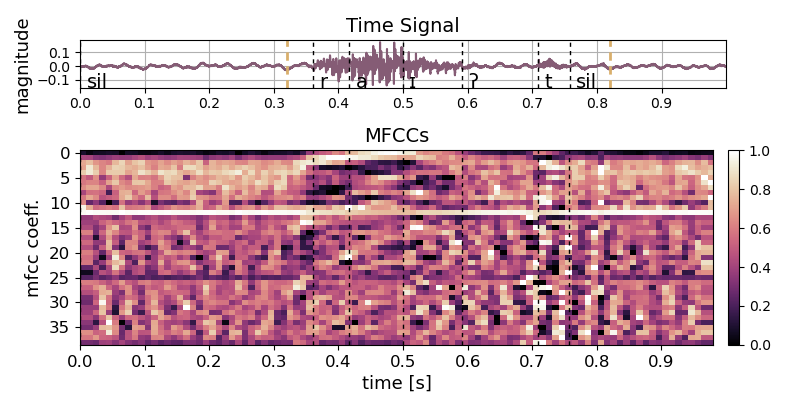
\includegraphics[width=0.6\textwidth]{../3_signal/figs/signal_mfcc_showcase_mfcc39_right0.png} \end{figure}
\end{frame}


\begin{frame}
  \frametitle{Onset Detection}
  \begin{itemize}
    \item Two kinds of onset detection method:
    \begin{itemize}
      \item Keyword onset detection:
        \begin{itemize}
          \item used in order to find exact start of keyword in audiofile
          \item applied for the extraction of data examples of restricted time length (\SI{500}{\milli\second}).
        \end{itemize}
      \item Online onset detection:
        \begin{itemize}
          \item applied in the game to indicate whether a keyword is present.
        \end{itemize}
    \end{itemize}
  \end{itemize}
\end{frame}

\begin{frame}
  \frametitle{Keyword Onset Detection}
  \vspace{-0.5cm}
  \begin{figure} 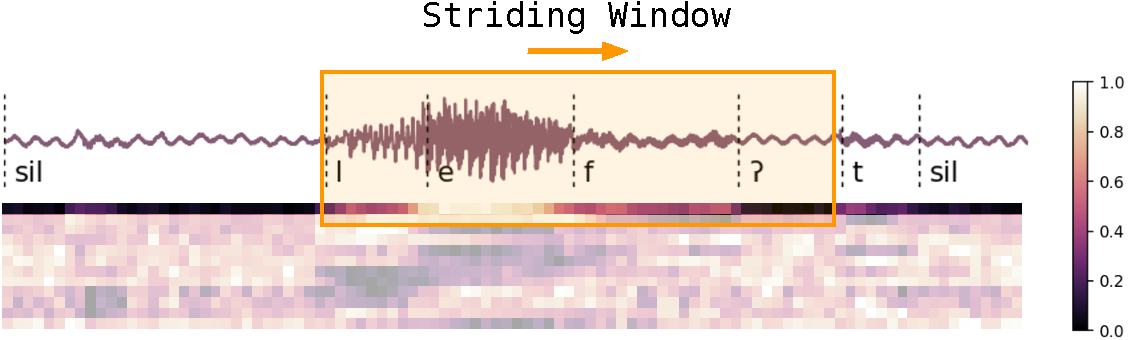
\includegraphics[width=0.8\textwidth]{../3_signal/figs/signal_onset_window.pdf} \end{figure}
  \begin{figure} 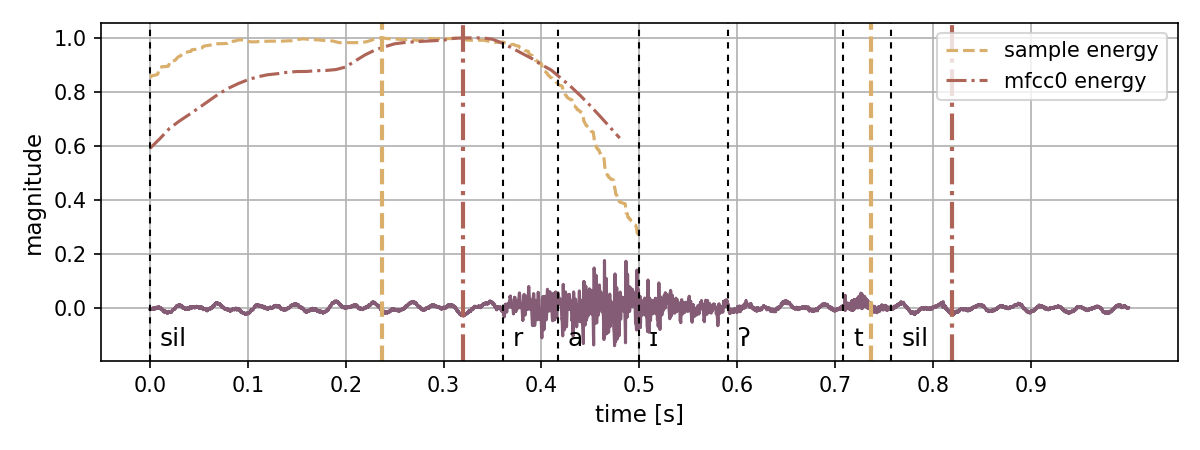
\includegraphics[width=0.8\textwidth]{../3_signal/figs/signal_onset_showcase_right0.png} \end{figure}
\end{frame}